\section{S\&P 500}

\begin{enumerate}[label=\textbf{\Alph*}.]
    \item Fit a Gaussian with ML.

    For a Gaussian, $P(R) = \frac{1}{\sqrt{2\pi}\sigma} e^{-\frac{(R-\mu)^2}{2\sigma^2}}$.

    Calculate the negative log likelihood:

    \begin{align*}
        L &= \prod P(R_i) \\
        -\ln(L) &= -\sum \ln P(R_i) \\
        -\ln(L) &= -\sum \ln\left(\frac{1}{\sqrt{2\pi}\sigma} e^{-\frac{(R_i-\mu)^2}{2\sigma^2}}\right) \\
        -\ln(L) &= \sum\left( -\ln \left(\frac{1}{\sqrt{2\pi}\sigma}\right) - \ln e^{-\frac{(R_i-\mu)^2}{2\sigma^2}}\right) \\
        -\ln(L) &= \sum\left(\ln \left(\sqrt{2\pi}\sigma\right) + \frac{(R_i-\mu)^2}{2\sigma^2}\right) \\
    \end{align*}

    This can be minimized computationally (see the code). Doing so gives:

    $$\mu_0=0.000108, \sigma_0=0.0129$$

    \item Fit a Laplace distribution, also with ML.

    Our new distribution, $f(R) = \frac{1}{2B} e^{-\frac{|R-A|}{B}}$.
    Calculate the negative log likelihood:

    \begin{align*}
        L &= \prod f(R_i) \\
        -\ln(L) &= -\sum \ln f(R_i) \\
        -\ln(L) &= -\sum \ln\left(\frac{1}{2B} e^{-\frac{|R-A|}{B}}\right) \\
        -\ln(L) &= \sum\left(- \ln\left(\frac{1}{2B}\right) - \ln e^{-\frac{|R-A|}{B}}\right) \\
        -\ln(L) &= \sum\left(\ln\left(2B\right) + \frac{|R-A|}{B}\right) \\
    \end{align*}

    Again, minimize computationally, which gives:

    $$A_0=0.000488, B_0=0.00764$$

    \newpage
    \item Plot a histogram on a log scale of the $R_i$ and overlay each best fit. Which one looks better?

    I'd say the Laplace distribution looks better.
    \begin{figure}[H]
        \begin{center}
            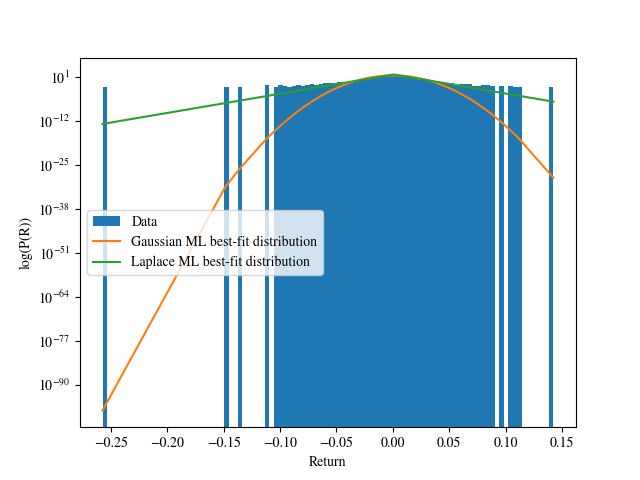
\includegraphics[width=0.9\textwidth]{images/q1_return_hist.png}
        \end{center}
    \end{figure}
    \newpage
    \item Simulate the growth of a \$100 investment using the best-fit Laplace, Gaussian, and drawing returns from the data.

    See code for how the simulation was done. Here, it looks like the Gaussian model is better.
    \begin{figure}[H]
        \begin{center}
            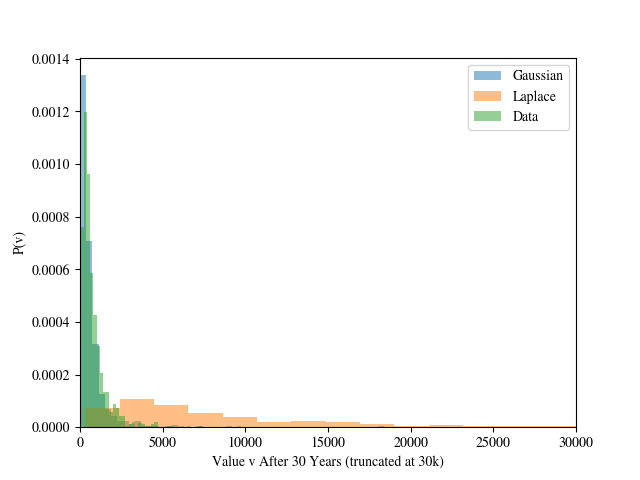
\includegraphics[width=0.9\textwidth]{images/q1_generator_comparison.png}
        \end{center}
    \end{figure}

\end{enumerate}
